\documentclass{article}

\usepackage[left=1.8in,right=1.8in,top=.6in,bottom=1in]{geometry}

\usepackage{assumptionsofphysics}
\usepackage{tikz}
\usetikzlibrary{positioning}
\usepackage{hyperref}
\hypersetup{
	colorlinks=true,
	citecolor=blue,
	urlcolor=blue,
	linkcolor=blue
}
\frenchspacing

\newcommand{\marginleft}[1] {\reversemarginpar\marginpar{#1}}
\newcommand{\marginright}[1] {\normalmarginpar\marginpar{#1}}

\def\ordinals{\textbf{ORD}}
\def\cardinals{\textbf{CRD}}

\def\ordless{\prec}
\def\ordleq{\preceq}
\def\ordeq{\sim}
\def\ordgeq{\succeq}

\def\crdleq{\hookrightarrow}
\def\crdeq{\leftrightarrow}
\def\crdgeq{\hookleftarrow}


\title{Bare minimum: set theory}

\date{\vspace{-5ex}}
\begin{document}

\maketitle


\begin{abstract}
This note presents a condensed summary of set theory which can function as a crash course, refresher and/or reference. Bare minima are meant to give a rough overview, by no means complete, of the subject to the intellectually curious, particularly in the context of foundational questions in physics. This work is part of Assumptions of Physics (\url{https://assumptionsofphysics.org}), a project that aims to identify a handful of physical principles from which the basic laws can be rigorously derived.
\end{abstract}


\section{Introduction}

Set theory is important for those working on Assumptions of Physics for at least three reasons. First, it is a foundational framework in mathematics. Second, it showcases a successful attempt at concept generalization. Third, it shows how a formal system is bootstrapped.

There are roughly two branches of set theory: naive and axiomatic. Naive set theory is built on intuitive concepts, and as such is not fully formalized and is open to potential paradoxes. Axiomatic set theory provides a fully formalized axiomatic system that aims to close those problems. We will start with naive set theory, which is the best setting for defining all the basic notions and getting a sense of how the framework works. Then we will turn our attention to axiomatic set theory to get a sense of what problems it solves and how, and whether those solutions mesh with foundational goals in physics.

For more details on set theory, see for example \cite{pinter2014book, settheory-tutorial}.

\section{Naive set theory}

We take sets and elements as primitive objects, with no formal definition. This is the only difference between naive and axiomatic set theory, therefore all the formal definitions that follow apply to both. A \textbf{set} $A$ is a collection of elements. If an element $e$ belongs to the set we say $e$ \textbf{is in} $A$, noted $ e 
\in A$. A set $A$ can be defined by listing the elements, noted $A = \{ e_1, e_2, e_3 \}$. A set $A$ can be defined by specifying how to build the elements through a rule (i.e. predicate) $P(e)$, and is noted $A = \{e \, | \,  P(e) \}$. The rule may include symbols like for all $\forall$, exists $\exists$, logical connectors AND $\AND$, OR $\OR$ and NOT $\NOT$.

\begin{defn}[Common sets]
	 The \textbf{empty set}
	 \marginleft{Common sets: $\emptyset$, $\{a\}$, $\mathbb{N}$, $\mathbb{Z}$, $\mathbb{Q}$, $\mathbb{R}$, $\mathbb{C}$}
	  $\emptyset$ is the set with no elements. A \textbf{singleton} is the set of a single element $\{a\}$.
	 The \textbf{set of natural numbers} $\mathbb{N} = \{ 0, 1, 2, ... \}$. The \textbf{set of positive natural numbers} $\mathbb{N}^+ = \{n \in \mathbb{N} \, | \, n > 0\}$. The \textbf{set of integer numbers} $\mathbb{Z} = \{ ... , -2, -1, 0, +1, +2, ...\}$. The \textbf{set of rational numbers} $\mathbb{Q}$. The \textbf{set of real numbers} $\mathbb{R}$. The \textbf{set of complex numbers} $\mathbb{C}$. A \textbf{universe} $U$ is the set that, within a specific context, contains all entities under study.
\end{defn}

\subsection{Basic definitions}

\marginright{~\\
	\def\setA{ (-1,0) circle (2) }
	\def\setB{ (1,0) circle (2) }
	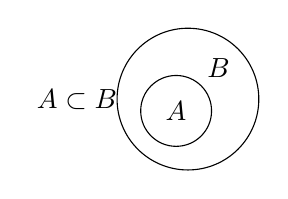
\begin{tikzpicture}[scale = 0.3]
		\draw (0,0) circle (3); 
		\draw (-0.5,-0.5) circle (1.5);
		\node at (-4.7,0) {$A \subset B$};
		\node at (-0.5,-0.5) {$A$};
		\node at (1.3,1.3) {$B$};
	\end{tikzpicture} 
}

\begin{defn}[Set relationships]
	Let $A$ and $B$ be two sets. \marginleft{Subset, superset: $\subseteq$, $\supseteq$} If all elements in $A$ are also contained in $B$, we say $A$ is a \textbf{subset} of $B$, noted $A \subseteq B$. In this case, we also say $B$ is a \textbf{superset} of $A$, noted $B \supseteq A$. Additionally, if $B$ contains elements that $A$ does not contain, we say $A$ is a \textbf{strict subset} of $B$, noted $A \subset B$, and $B$ is a \textbf{strict superset} of $A$, noted $B \supset A$. If the two sets contain exactly the same elements, then we say the sets are \textbf{equal}, noted $A = B$. If the two sets have no element in common they are said to be \textbf{disjoint}.
\end{defn}

\begin{defn}[Power set]
	Given a set $A$, its \textbf{power set}, \marginleft{Power set:\\ $\mathcal{P}(A)$, $2^{A}$} noted $\mathcal{P}(A)$ or $2^{A}$, is the set of all subsets of $A$. That is, $\mathcal{P}(A) = \{B \, | \, B \subseteq A \}$.
\end{defn}

\marginright{
	~\\
	\def\setA{ (-1,0) circle (2) }
	\def\setB{ (1,0) circle (2) }
	\vspace{1pt}
	\begin{tikzpicture}[scale = 0.3]
		\filldraw[black!10] \setA;
		\filldraw[black!10] \setB;
		\draw \setA; 
		\draw \setB;
		\node at (-4.7,0) {$A\!\cup \! B$};
	\end{tikzpicture} 
	\vspace{1pt}
	\begin{tikzpicture}[scale = 0.3]
		\begin{scope}
			\clip \setA;
			\filldraw[black!10] \setB;
		\end{scope}
		\draw \setA; 
		\draw \setB;
		\node at (-4.7,0) {$A\!\cap \! B$};
	\end{tikzpicture} 
	\vspace{1pt}
	\begin{tikzpicture}[scale = 0.3]
		\filldraw[black!10] \setA;
		\filldraw[white] \setB;
		\draw \setA; 
		\draw \setB;
		\node at (-4.7,0) {$A\!\setminus \! B$};
	\end{tikzpicture}
	\def\setU{ (-3,-2) rectangle (3,2) }
	\def\setA{ (0,0) circle (1.8) }
	\begin{tikzpicture}[scale = 0.3] 
		\filldraw[black!10] \setU;
		\filldraw[white] \setA;
		\draw \setU;
		\draw \setA;
		\node at (-5.3,0) {$A^{\complement}$};
	\end{tikzpicture} 
}

\begin{defn}[Set operations]
	We define \marginleft{Set operations: $\cup$, $\cap$, $\setminus$, $^{\complement}$} the following operations between two sets $A$ and $B$:
	\begin{description}
		\item[Union.]Noted $A \cup B$, the union of $A$ and $B$ is the set of all elements that are contained by $A$, $B$ or both.
		\item[Intersection.] Noted $A \cap B$, the intersection of $A$ and $B$ is the set of all elements that are contained by both.
		\item[Set difference (or relative complement).] Noted $A \setminus B$, $A$ minus $B$ is the set of all elements in $A$ that are not contained by $B$.
		\item[Complement (or absolute complement).] Noted $A^{\complement}$, represents all elements that are not contained in $A$. Note that this operation is context specific: we need to know that, within a certain context, $U$ is the set of all elements under study; then the complement of $A \subseteq U$ is $A^{\complement} = U \setminus A$.
	\end{description}

	Let $\mathcal{A} \subseteq \mathcal{P}(A)$ be a set of subsets of $A$. The operations of union $\bigcup\limits_{A \in \mathcal{A}} A$ and intersection $\bigcap\limits_{A \in \mathcal{A}} A$ can be extended to span all elements.
\end{defn}

\begin{defn}[Ordered pair]
	Given two \marginleft{Ordered pair: $(a, b)$} elements $a$ and $b$, the \textbf{ordered pair} $(a, b)$ specifies two objects in that order. That is $(a, b) \neq (b, a)$. This can be constructed by setting $(a, b) = \{ \{a\}, \{a, b\}\}$.
\end{defn}

\marginright{~\\
	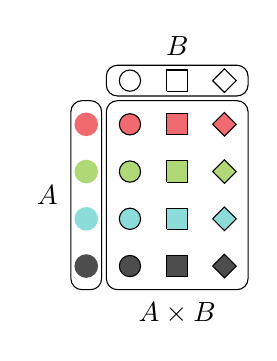
\begin{tikzpicture}[scale = 0.3] 
		\node at (-2.5,-4) {$A$};
		\node at (3,2.3) {$B$};
		\draw[rounded corners] (0,0.2) rectangle (6,1.5);
		\draw[rounded corners] (-0.2,0) rectangle (-1.5,-8);
		\draw[rounded corners] (0,0) rectangle (6,-8);
		
		\def\circlepath{circle (0.45)}
		\def\rectanglepath{ ++(-0.45,-0.45)  -- ++(0,0.9)  -- ++(0.9,0) -- ++(0,-0.9) -- ++(-0.9,0)}
		\def\diamondpath{ ++(-0.5,0)  -- ++(0.5,0.5)  -- ++(0.5,-0.5) -- ++(-0.5,-0.5) -- ++(-0.5,0.5)}
		
		% B elements
		\draw (1,0.85) \circlepath;
		\draw (3,0.85) \rectanglepath;
		\draw (5,0.85) \diamondpath;
		
		\definecolor{a}{rgb}{0.945, 0.415, 0.439}
		\definecolor{b}{rgb}{0.694, 0.847, 0.466}
		\definecolor{c}{rgb}{0.549, 0.862, 0.854}
		\definecolor{d}{rgb}{0.301, 0.301, 0.301}
		
		% A elements
		\fill[a] (-0.85, -1) circle (0.5);
		\fill[b] (-0.85, -3) circle (0.5);
		\fill[c] (-0.85, -5) circle (0.5);
		\fill[d] (-0.85, -7) circle (0.5);

		% AxB elements
		\filldraw[fill=a] (1, -1) \circlepath;
		\filldraw[fill=b] (1, -3) \circlepath;
		\filldraw[fill=c] (1, -5) \circlepath;
		\filldraw[fill=d] (1, -7) \circlepath;
		\filldraw[fill=a] (3, -1) \rectanglepath;
		\filldraw[fill=b] (3, -3) \rectanglepath;
		\filldraw[fill=c] (3, -5) \rectanglepath;
		\filldraw[fill=d] (3, -7) \rectanglepath;
		\filldraw[fill=a] (5, -1) \diamondpath;
		\filldraw[fill=b] (5, -3) \diamondpath;
		\filldraw[fill=c] (5, -5) \diamondpath;
		\filldraw[fill=d] (5, -7) \diamondpath;

		\node at (3,-9) {$A \times B$};
	\end{tikzpicture} 
}
\begin{defn}[Cartesian product]
	Given two sets \marginleft{Cartesian product: $\times$}  $A$ and $B$, the \textbf{Cartesian product} $A \times B = \{ (a,b) \, | \, \forall a \in A, b \in B \}$ is the set of all possible ordered pairs between the elements of $A$ and $B$.
\end{defn}

\begin{defn}[Disjoint union]
	Let $A$ and $B$ be two sets. The disjoint union $A \sqcup B$ is the union where the elements of the sets are always treated as distinct. That is, given $A \sqcup B = (\{0\} \times A ) \cup ( \{1\} \times B )$.
\end{defn}

\begin{remark}
	Ordered pairs and disjoint unions exemplify the effort in set theory to construct \emph{all objects} starting from just two primitives: set and set inclusion. The downside is that the constructions do not map exactly to our intuition. For example, we still think an ordered pair as a set, so we want to write $b \in (a, b)$, though, looking at the definition $b$ itself is not directly a member of $(a, b)$.
\end{remark}

\subsection{Relations and functions}

\begin{remark}
	Relations provide a common foundation for functions (i.e. the relation is the set of pairs $(x, f(x))$ ), equivalences and order (i.e. the relation is the set of pairs $(a, b)$ such that $a=b$ or $a\leq b$ respectively). This exemplifies the effort in set theory to find general structures.
\end{remark}

\marginright{~\\
	\begin{tikzpicture}[scale = 0.3] 
		\node at (-2.5,-4) {$A$};
		\node at (3,2.3) {$B$};
		\draw[rounded corners] (0,0.2) rectangle (6,1.5);
		\draw[rounded corners] (-0.2,0) rectangle (-1.5,-8);
		\draw[rounded corners] (0,0) rectangle (6,-8);
		
		\def\circlepath{circle (0.45)}
		\def\rectanglepath{ ++(-0.45,-0.45)  -- ++(0,0.9)  -- ++(0.9,0) -- ++(0,-0.9) -- ++(-0.9,0)}
		\def\diamondpath{ ++(-0.5,0)  -- ++(0.5,0.5)  -- ++(0.5,-0.5) -- ++(-0.5,-0.5) -- ++(-0.5,0.5)}
		
		% B elements
		\node at (1,0.85) {
\includegraphics[scale=0.25]{cat.png}};
		\node at (3,0.85) {
\includegraphics[scale=0.25]{dog.png}};
		\node at (5,0.85) {
\includegraphics[scale=0.25]{swan.png}};
		
		\definecolor{a}{rgb}{1.0, 1.0, 1.0}
		\definecolor{b}{rgb}{1, 0.509, 0}
		\definecolor{c}{rgb}{0.45, 0.225, 0}
		\definecolor{d}{rgb}{0, 0, 0}
		
		% A elements
		\filldraw[fill=a] (-0.85, -1) circle (0.5);
		\fill[b] (-0.85, -3) circle (0.5);
		\fill[c] (-0.85, -5) circle (0.5);
		\fill[d] (-0.85, -7) circle (0.5);
		
		% AxB elements
		\node at (1, -1) {$\checkmark$};
		\node at (1, -3) {$\checkmark$};
		\node at (1, -5) {};
		\node at (1, -7) {$\checkmark$};
		\node at (3, -1) {$\checkmark$};
		\node at (3, -3) {};
		\node at (3, -5) {$\checkmark$};
		\node at (3, -7) {$\checkmark$};
		\node at (5, -1) {$\checkmark$};
		\node at (5, -3) {};
		\node at (5, -5) {};
		\node at (5, -7) {$\checkmark$};
		
		\node at (3,-9) {$R$};
	\end{tikzpicture} 
	
	\begin{tikzpicture}[scale = 0.3] 
		\node at (-2.5,-3) {$B$};
		\node at (4,2.3) {$A$};
		\draw[rounded corners] (0,0.2) rectangle (8,1.5);
		\draw[rounded corners] (-0.2,0) rectangle (-1.5,-6);
		\draw[rounded corners] (0,0) rectangle (8,-6);
		
		\def\circlepath{circle (0.45)}
		\def\rectanglepath{ ++(-0.45,-0.45)  -- ++(0,0.9)  -- ++(0.9,0) -- ++(0,-0.9) -- ++(-0.9,0)}
		\def\diamondpath{ ++(-0.5,0)  -- ++(0.5,0.5)  -- ++(0.5,-0.5) -- ++(-0.5,-0.5) -- ++(-0.5,0.5)}
		
		% B elements
		\node at (-0.85, -1) {
\includegraphics[scale=0.25]{cat.png}};
		\node at (-0.85, -3) {
\includegraphics[scale=0.25]{dog.png}};
		\node at (-0.85, -5) {
\includegraphics[scale=0.25]{swan.png}};
		
		\definecolor{a}{rgb}{1.0, 1.0, 1.0}
		\definecolor{b}{rgb}{1, 0.509, 0}
		\definecolor{c}{rgb}{0.45, 0.225, 0}
		\definecolor{d}{rgb}{0, 0, 0}
		
		% A elements
		\filldraw[fill=a] (1,0.85) circle (0.5);
		\fill[b] (3,0.85) circle (0.5);
		\fill[c] (5,0.85) circle (0.5);
		\fill[d] (7,0.85) circle (0.5);
		
		% AxB elements
		\node at (1, -1) {$\checkmark$};
		\node at (3, -1) {$\checkmark$};
		\node at (5, -1) {};
		\node at (7, -1) {$\checkmark$};
		\node at (1, -3) {$\checkmark$};
		\node at (3, -3) {};
		\node at (5, -3) {$\checkmark$};
		\node at (7, -3) {$\checkmark$};
		\node at (1, -5) {$\checkmark$};
		\node at (3, -5) {};
		\node at (5, -5) {};
		\node at (7, -5) {$\checkmark$};
		
		\node at (4,-7) {$R^{-1}$};
	\end{tikzpicture} 
	
}
\begin{defn}[Binary relation]
	Given a set $A$, \marginleft{Binary\\ relation: $aRb$} called \textbf{domain}, and a set $B$, called \textbf{codomain}, a \textbf{binary relation} is a set $R \subseteq A \times B$ of ordered pairs. We say $a$ is \textbf{$R$-related} to $b$, noted $aRb$ if $(a,b) \in R$. If $A=B$ (i.e. domain and codomain coincide) the relation is said to be \textbf{homogeneous}, \textbf{heterogeneous} if not.
\end{defn}

	
\begin{defn}[Image and preimage]
	If $X \subseteq A$, \marginleft{Image and\\ preimage} the \textbf{image of $X$ under $R$} is the set of all elements in $B$ that are related to at least one element in $X$. The \textbf{image of $R$} is the set of all elements in $B$ that are related to at least one element in $A$ (i.e. the image of the full set $A$).
	
	If $Y \subseteq B$, the \textbf{preimage of $Y$ under $R$} is the set of all elements in $A$ that are related to at least one element in $Y$. The \textbf{preimage of $R$} is the set of all elements in $A$ that are related to at least one element in $B$ (i.e. the preimage of the full set $B$).
\end{defn}


\begin{defn}[Converse relationship]
	Given a relationship  \marginleft{Converse: $R^{-1}$} $R$ between $A$ and $B$, the \textbf{converse} or \textbf{inverse} relationship $R^{-1} \subseteq B \times A$ is the relationship where the order of the pairs (i.e. domain and codomain) is inverted. That is, $R^{-1} = \{ (b, a) \, | \, (a, b) \in R\}$.
\end{defn}

\begin{defn}[Relation properties]
	Let $R$ \marginleft{Relation properties} be a binary relation between $A$ and $B$. We define the following properties:
	\begin{description}
		\item[Functional or right-unique.] An element $a \in A$ is related to at most one element $b \in B$. That is, if $aRb$ and $aRc$ then $b = c$.
		\item[Injective or left-unique.] An element $b \in B$ is related to at most one element $a \in A$. That is, if $aRb$ and $cRb$ then $a = c$.
		\item[Serial or left-total.] Every element $a \in A$ is related to at least one element $b \in B$. That is, for each $a \in A$ there exists at least one $b \in B$ such that $aRb$. In this case, the preimage of $R$ is the whole $A$.
		\item[Surjective or right-total.] Every element $b \in B$ is related to at least one element $a \in A$. That is, for each $b \in B$ there exists at least one $a \in A$ such that $aRb$. In this case, the image of $R$ is the whole $B$.
	\end{description}
	From those basic properties, we define the following:
	\begin{description}
		\item[One-to-one.] Injective and functional (i.e. left-unique and right-unique).
		\item[One-to-many.] Injective and not functional (i.e. left-unique and not right-unique).
		\item[Many-to-one.] Not injective and functional (i.e. not left-unique and right-unique).
		\item[Many-to-many.] Not injective nor functional (i.e. not left-unique nor right-unique).
	\end{description}	
\end{defn}

\begin{defn}[Function]
	A \textbf{partial function} \marginleft{(Partial) \\ functions: \\ $f : A \to B$} $f : A \to B$ is a binary relationship between $A$ and $B$ that is functional (i.e. right-unique). The \textbf{graph} of the function $G \subset A \times B$ is the function expressed as ordered pairs. A \textbf{total function}, or simply a \textbf{function}, is a partial function that is also serial (i.e. left-total, defined on the whole domain). A function is \textbf{bijective} if it is injective and surjective.
	
	When the functional form $f(a)$ is known, this can be expressed as $a \mapsto f(a)$ (read ``$a$ maps to $f$ of $a$'').
\end{defn}

\begin{remark}
	Note that the domain and the codomain can be any set, including scalar products. Therefore $f : \mathbb{R} \times \mathbb{R} \to \mathbb{R}$ for which $(x,y) \mapsto \sqrt{x^2 + y^2}$ gives us the Euclidean norm of a two dimensional vector.
\end{remark}

\begin{defn}[Identity function]
	Given a set $A$, \marginleft{Identity: $\Id_A$} the identity function $\Id_A : A \to A$ is the function such that $\Id_A(a) = a$ for all $a \in A$.
\end{defn}

\begin{prop}[Inverse function]
	Let $f : A \to B$ \marginleft{Inverse: $f^{-1}$} be a function. The corresponding converse relationship $f^{-1}$ is a function if and only if $f$ is bijective. In this case $f^{-1} : B \to A$ is also bijective and is called the \textbf{inverse} of $f$.
\end{prop}

\begin{defn}[Image/preimage functions]
	Let $f : A \to B$ \marginleft{$f(X), f^{-1}(Y)$} be a function. This induces a relation $f : \mathcal{P}(A) \to \mathcal{P}(B)$ that associates each subset of $A$ to its image and a relation $f^{-1} : \mathcal{P}(B) \to \mathcal{P}(A)$ that associates each subset of $B$ with its preimage.
\end{defn}

\begin{prop}[Properties of image/preimage functions]
	The induced relations $f : \mathcal{P}(A) \to \mathcal{P}(B)$ and $f^{-1} : \mathcal{P}(B) \to \mathcal{P}(A)$ are functions and satisfy the following properties for all $\mathcal{A} \subseteq \mathcal{P}(A)$ and $\mathcal{B} \subseteq \mathcal{P}(B)$:
	\begin{enumerate}
		\item $f(\bigcup\limits_{U \in \mathcal{A}} U) = \bigcup\limits_{U \in \mathcal{A}} f(U)$
		\item $f^{-1}(\bigcup\limits_{V \in \mathcal{B}} V) = \bigcup\limits_{V \in \mathcal{B}} f^{-1}(V)$
		\item $f^{-1}(\bigcap\limits_{V \in \mathcal{B}} V) = \bigcap\limits_{V \in \mathcal{B}} f^{-1}(V)$
	\end{enumerate}
\end{prop}

\begin{remark}
	With abuse of notation, $f$ and $f^{-1}$ indicate both the function between elements and sets. Note that $f^{-1} : \mathcal{P}(B) \to \mathcal{P}(A)$ always exists even if $f$ is not bijective. Also note that the image of the intersection is not in general the intersection of the image, and how maps that preserve set theoretic structures (e.g. topologies and $\sigma$-algebras) are defined based on preimages.
\end{remark}

\begin{defn}[Fiber]
	Given \marginleft{Fiber} a function $f : A \to B$, the \textbf{fiber of $b \in B$ under $f$} is the subset of $A$ of where the function takes the value $b$. That is, the preimage $f^{-1}(\{b\})$ of the singleton. Fibers over real functions are also called \textbf{level sets}.
\end{defn}


\begin{defn}[Restriction]
	Let $f : A  \to B$ \marginleft{Restriction: $f|_C$} be a function and let $C \subseteq A$. Then the \textbf{restriction of $f$ over $C$} is the function $f|_C : C \to B$ such that $f|_C(c) = f(c)$ for all $c \in C$.
\end{defn}

\begin{defn}[Composition]
	Let $A$, $B$ and $C$ \marginleft{Function and relation composition: $R \circ S$, $f \circ g$} be three sets. Let $R$ be a binary relationship between $A$ and $B$ and $S$ be a binary relationship between $B$ and $C$. Then the \textbf{composition of $R$ and $S$} is the binary relationship $S \circ R \subseteq A \times C$ between $A$ and $C$ such that $(a, c) \in S \circ R$ if we can find $b \in B$ such that $aRb$ and $bSc$.
\end{defn}

\begin{remark}
	The order of composition follows those of functions: if $f : A \to B$ and $g : B \to C$, composition leads to $c = g(f(a)) = (g \circ f)(a)$.
\end{remark}

\begin{prop}[Composition properties]
	Relation composition \marginleft{Composition properties} follows the following properties:
	\begin{itemize}
		\item Composition is associative: $R \circ (T \circ S) = (R \circ T) \circ S$
		\item Converse of composition: $(R \circ S)^{-1} = S^{-1} \circ R^{-1}$
		\item Composition of functional/injective/serial/surjective relations is \\ functional/injective/serial/surjective.
		\item If $f : A \to B$ and $g : B \to C$ are (partial) functions, then $g \circ f$ is a (partial) function.
		\item Let $f : A \to B$ be a bijective function, then $f \circ f^{-1} = \Id_B$ and $f^{-1} \circ f = \Id_A$.
	\end{itemize}
\end{prop}

\begin{defn}[Sets of functions]
	The set \marginleft{Sets of functions: $B^A$} of all possible functions $f : A \to B$ is noted $B^A$.
\end{defn}

\begin{prop}
	Let $2 = \{0, 1\}$ denote a set with two elements. Then $\mathcal{P}(A)$ and $2^A$ are in one-to-one correspondence.
\end{prop}

\begin{remark}
	The notation for function sets is due to the cardinality. If $A$ has $n$ elements and $B$ has $m$ elements, each function is given by choosing an element of $B$ for each element of $A$, that is $m$ choices $n$ times, that is $m^n$. The power set is noted $2^A$ because each subset $U \subseteq A$ can be identified by a unique function $f : A \to \{0 , 1\}$, where for all $a\in A$ then $f(a)=0$ corresponds to $a \notin U$ and $f(a)=1$ corresponds to $a \in U$.
\end{remark}

\begin{defn}[Set closure under operations]
	Let $f : A_1 \times A_2 \times ... \times A_n \to B$ be an $n$-ary function. We say a set \textbf{$A$ is closed under $f$} if whenever the function is applied to elements of $A$ it returns an element of $A$. That is, $A \subseteq A_i$ for all $1\leq i \leq n$, $A \subseteq B$ and $f(A, A, ..., A) \subseteq A$.
\end{defn}

\begin{remark}
	For example, integers are closed under addition, subtraction and multiplication but are not closed under division. Most mathematical structures (groups, topologies, $\sigma$-algebras, vector spaces, ...) define sets closed under some operations.
\end{remark}


\subsection{Indexed families and sequences}

\begin{defn}[Families]
	An \textbf{indexed family}, \marginleft{Families, sequences: $\{x_i\}_{i \in I}$, $\{x_i\}_{i=1}^{\infty}$} or simply a \textbf{family}, $\{x_i\}_{i \in I}$ is a collection of elements identified by an \textbf{index set} $I$. More formally, an indexed family is a tuple $( X, I, x )$ where $X$ and $I$ are sets and $x: I \to X$ is a function such that $i \mapsto x_i$. A \textbf{sequence} is a family for which the index set is a contiguous interval of natural numbers. A \textbf{finite sequence} of $n$ elements is noted $\{x_i\}_{i=1}^{n}$ while an \textbf{infinite sequence} is noted $\{x_i\}_{i=1}^{\infty}$.
\end{defn}

\begin{defn}[Operations on families of sets]
	Let $\{A_i\}_{i \in I}$ \marginleft{$\bigcap\limits_{i \in I} A_i $, $\bigcup\limits_{i \in I} A_i$} be a family of sets, the operations of intersection $\bigcap\limits_{i \in I} A_i $ and union $\bigcup\limits_{i \in I} A_i$ can be extended to span all members.
\end{defn}

\begin{defn}[Set-theoretic limit]
	Let $\{A_i\}_{i=1}^{\infty}$ \marginleft{Set limit: \\ $\lim\limits_{i \to \infty} A_i = A$} be a sequence of sets. We define the \textbf{limit infimum} as $\liminf\limits_{i \to \infty} A_i = \bigcup\limits_{i \geq 1}\bigcap\limits_{j \geq i} A_j$ and the \textbf{limit supremum} as $\limsup\limits_{i \to \infty} A_i = \bigcap\limits_{i \geq 1}\bigcup\limits_{j \geq i} A_j$. If the two are equal to the same set then we say the sequence \textbf{converges}, the \textbf{set-theoretic limit} $\lim\limits_{i \to \infty} A_i = A$ exists and it is equal to that set.
\end{defn}

\marginright{~\\
	\def\setA{ (-1,0) circle (2) }
	\def\setB{ (1,0) circle (2) }
	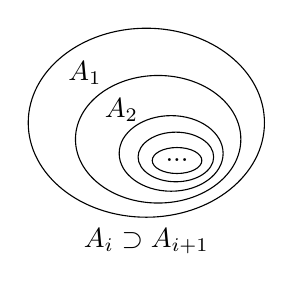
\begin{tikzpicture}[scale = 0.3]
		\draw (0,0) ellipse (5 and 4); 
		\draw (0.5,-0.7) ellipse (3.5 and 2.7);
		\draw (1.05,-1.3) ellipse (2.2 and 1.6);
		\draw (1.25,-1.45) ellipse (1.6 and 1.05);
		\draw (1.3,-1.6) ellipse (1.05 and 0.55);
		\node at (0,-5) {$A_i \supset A_{i+1}$};
		\node at (-2.6, 2.1) {$A_1$};
		\node at (-1.05,0.55) {$A_2$};
		\node at (1.3,-1.6) {$...$};
	\end{tikzpicture} 
}
\begin{defn}[Monotone sequence]
	A \textbf{monotone sequence} \marginleft{Monotone sequence: \\ $A_1 \subseteq A_2 \subseteq ...$\\ $A_1 \supseteq A_2 \supseteq ...$} is a sequence of sets $\{A_i\}_{i=1}^{\infty}$ where each set is a subset (or superset) of the preceding. More specifically, we distinguish four cases:
	\begin{description}
		\item[Increasing] when $A_i \subseteq A_{i+1}$ for all $i \geq 1$
		\item[Decreasing] when $A_i \supseteq A_{i+1}$ for all $i \geq 1$
		\item[Strictly increasing] when $A_i \subset A_{i+1}$ for all $i \geq 1$
		\item[Strictly decreasing] when $A_i \supset A_{i+1}$ for all $i \geq 1$
	\end{description}
\end{defn}

\begin{prop}[Monotone convergence]
	All monotone \marginleft{Monotone convergence} sequences converge. For increasing sequences the limit is given by $\lim\limits_{i \to \infty} A_i = \bigcup\limits_{i \geq 1} A_i$, while for decreasing sequences  the limit is given by $\lim\limits_{i \to \infty} A_i = \bigcap\limits_{i \geq 1} A_i$.
\end{prop}

\subsection{Homogeneous relations, equivalences and orders}

\begin{remark}
	We will cover the notions of orders that are necessary for the definition of ordinal and cardinal numbers. Orders will be treated more in detail in a Bare Minimum dedicated to order theory.
\end{remark}

\begin{defn}[Homogeneous relation properties]
	Let $R \subseteq A \times A$ \marginleft{Reflexivity, symmetry, transitivity, ...} be a homogeneous binary relation between $A$ and itself. We define the following properties:
	\begin{description}
		\item[Reflexive.] Every element $a \in A$ is related to itself. That is, $aRa$ for all $a \in A$.
		\item[Irreflexive.] No element $a \in A$ is related to itself. That is, $aRa$ for no $a \in A$.
		\item[Symmetric.] If $a$ is related to $b$, then $b$ is related to $a$. That is, if $aRb$ then $bRa$.
		\item[Antisymmetric.] If $a$ is related to $b$ and $b$ is related to $a$, then $a$ and $b$ are the same element. That is, if $aRb$ and $bRa$ then $a=b$.
		\item[Transitive.] If $a$ is related to $b$ and $b$ is related to $c$, then $a$ is related to $c$. That is, if $aRb$ and $bRc$ then $aRc$.
		\item[Total.] Given two distinct elements, one is related to the other.That is, given $a \neq b$, either $aRb$ or $bRa$. (This has no relation to left/right-total)
	\end{description}
	
\end{defn}

\begin{defn}[Orders and equivalence]
	A \textbf{partial order} \marginleft{Order, equivalence: $\leq$, $<$, $\equiv$} (noted for example $\leq$, $\lesssim$, $\preceq$)  is a homogeneous binary relationship that is reflexive, antisymmetric and transitive. A \textbf{linear order} or \textbf{total order} is an order that is total. An order is \textbf{strict} (noted for example $<$, $\prec$) if it is irreflexive instead of reflexive.
	
	An \textbf{equivalence relation} (noted for example $\equiv$, $\sim$) is a homogeneous binary relationship that is reflexive, symmetric and transitive.
\end{defn}


\begin{defn}[Partitions]
	A \textbf{partition} \marginleft{Partitions} of a set $A$ is a collection $P \subset \mathcal{P}(A)$ of disjoint subsets that cover all of $A$. That is:
	\begin{enumerate}
		\item $\bigcup\limits_{B \in P} B = A$
		\item $B \cap C = \emptyset$ for all $B, C \in P$ where $B \neq C$
	\end{enumerate}
\end{defn}


\begin{defn}[Equivalence classes and quotient set]
	Let $A$ \marginleft{Eq. classes and quotient set: \\ $[a]_{\sim}, a_{/\sim}, A_{/\sim}$} be a set and $\sim$ an equivalence relation on $A$. Let $a \in A$. The \textbf{equivalence class of $a$ by $\sim$} is the set $[a]_{\sim} = a_{/\sim} = \{b \in A \, | \, b \sim a \}$ of all the elements of $A$ equivalent to $a$. The \textbf{quotient set of $A$ by $\sim$} $A_{/\sim} = \{ a_{/\sim} \, | \, a \in A \}$  is the set of all of the equivalence classes by $\sim$.
\end{defn}

TODO: diagram

\begin{prop}[Quotient sets are partitions]
	Every quotient set is a partition, and every partition is a quotient set. That is, let $A$ be a set and $\sim$ an equivalence class, then $A_{/\sim}$ is a partition. Conversely, let $P$ be a partition of $A$, then $\sim \; = \{ (a,b) \, | \, a, b \in X \text{ for some } X \in P \} $ is an equivalence relation and $A_{/\sim} = P$.
\end{prop}

\begin{defn}
	Given a function $f : A \to B$ the \textbf{equivalence relation determined by $f$} is the relation $R_f = \{ (a_1, a_2) \, | \, f(a_1) = f(a_2) \}$.
\end{defn}

\begin{prop}[Function canonical decomposition]
	Every function $f : A \to B$ can be written as the composition $f = t \circ s \circ r$ of the following three functions:
	\begin{description}
		\item[$r : A \to A_{/R_f}$] defined as $a \mapsto [a]_{R_f}$; this function is surjective
		\item[$s : A_{/R_f} \to f(A)$] defined as $[a]_{R_f} \mapsto f(a)$; this function is bijective
		\item[$t : f(A) \to B$] defined as $t(b) = b$; this function is injective.
	\end{description}
\end{prop}

\begin{remark}
	All the above concepts are of general use in all areas of mathematics. Note that they are all constructed on two primitives: the notion of sets and of set inclusion.
\end{remark}

\section{Axiomatic set theory}

Axiomatic set theory was introduced to eliminate some technical problems that would make naive set theory inconsistent. There is no single approach and there is no single set of axioms. For example, constructive set theory, as all constructive mathematics, rejects ``nonconstructive proofs'' in which the existence of an object is proved with no explicit algorithm as to how to construct it. This will lead to different choices than the ones outlined here. Much of the work on the foundations of mathematics in set theory is to clarify the relationship between the axioms: which ones are required to get certain results, which ones are independent and which ones are inconsistent.

This is an important insight for those working on Assumptions of Physics: the foundations of mathematics are not absolute. We have to be conscious of the consequences of those choices and understand whether they are suitable for the foundations of physics.

\subsection{Paradoxes}

While they are generally called paradoxes, the following are really contradictions and that is why axiomatic set theory needs to avoid them. The first type of paradoxes for naive set theory arises from the use of natural language and the meaning of the words, typically when this is self-referential.

\textbf{Berry's paradox}. Consider the expression ``the smallest positive integer not definable in under sixty letters.'' Given that there are only twenty-six letters in the English language, there are finitely many phrases under sixty letters and therefore only finitely many integers can be defined in under sixty letters. Therefore there are integers not definable under sixty letters and, since the integers are ordered, there will be a least one. However, the above expression contains fifty-seven letters. We have a contradiction.

This type of paradoxes is solved by restricting to symbolic expressions of a formal language, such as predicate logic. The consequence is that, at the foundational level, mathematics does not keep track of what the symbols mean.

The second type of paradoxes is purely logical, so they can be constructed in the formal system.

\textbf{Russell's paradox}. Let $R$ be the set of all sets that do not contain themselves. That is, $R=\{ x \, | \, x \notin x\}$. Suppose $R \notin R$ then, by definition, $R \in R$. Suppose $R \in R$ then, by definition, $R \notin R$. We have a contradiction.

These are solved by carefully specifying the rules that are allowed for the creation of sets, by picking the ``right'' axioms. Part of the solution revolves around the following concepts.

%https://en.wikipedia.org/wiki/Zermelo%E2%80%93Fraenkel_set_theory

%https://en.wikipedia.org/wiki/Von_Neumann–Bernays–Gödel_set_theory

\subsection{Classes, sets and elements}

A \textbf{class} \marginright{ ~\\
		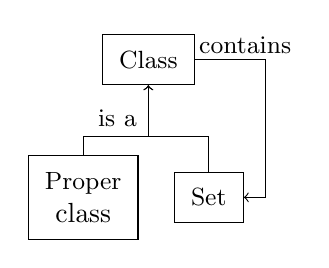
\begin{tikzpicture}[scale = 0.3]
		\node [draw, inner sep=6, rectangle] (class) {\small Class};
		\node [below=.3 of class] (middle) {};
		\node [below=1.3 of class] (lower) {};
		\node [draw, inner sep=6, rectangle, align=center, left=0 of lower] (pclass) {\small Proper \\ class};
		\node [draw, inner sep=6, rectangle, right=.2 of lower] (set) {\small Set};
		\draw[->] (pclass.north) -| ++(0,.8) -|  (class.south);	
		\draw[->] (set.north) -| ++(0,1.5) -|  (class.south);	
		\draw[->] (class.east) -| ++(3,0) |-  (set.east);	
		 %++(0,-1) -|
		\node [left=-0.1 of middle] (isa) {\small is a};
		\node at (4.1,.6) (contains) {\small contains};
	\end{tikzpicture} 
}  is any collection, therefore \textbf{sets are classes}. Some classes are not sets. These are called \textbf{proper classes} and are exactly the collections that cannot be elements of a class. Therefore, sets are classes that can be contained by other classes, while proper classes cannot. The difference between sets and proper classes is not in what they contain but in whether they can be contained. Proper classes are ``too large'' to be sets in the following sense: given a class $A$, if we can find a set $B$ that contains all elements of $A$, then $A$ will be a set as well. Therefore proper classes can never be subclasses of sets, they are bigger than all sets. The class of all sets, for example, is a proper class. So is the class of all cardinal numbers.

Note that axiomatic set theory does not distinguish between objects that can or cannot contain other objects. All elements are classes, all elements can, in principle, contain something. In fact, since equality of two objects coincides on whether they have the same elements, two objects must contain something different to be different. Numbers will be constructed as sets starting from the empty set. As a consequence, the proposition $3 \in 4$ is valid, and happens to be true if $3$ and $4$ are naturals, though it is not true if $3$ and $4$ are reals. From the perspective of Assumptions of Physics, this is not great as the framework allows propositions that are not physically meaningful. Radically different approaches to the foundations of mathematics (e.g. through category theory) do not exhibit this particular problem, though they exhibit others (e.g. identity of an object can be defined only up to its relationships with other objects).

\subsection{Axiomatization}

One strategy for the axiomatization of set theory, refered to as Zermelo–Fraenkel (ZFC), only defines sets. The C in ZFC stands for the addition of the axiom of choice. It avoids paradoxes by restricting set construction to subsets only. Proper classes are not objects that live in the framework.

Another strategy, refered to as von Neumann–Bernays–Gödel (NBG), starts by defining classes and then defines sets as those classes that can be elements of classes. It avoids paradoxes by restricting set construction on predicates over sets. Since a proper class cannot be an element, if the definition creates a contradiction for an item $x$ (i.e. we have both $x \in S$ and $x \notin S$) then it must be that the element $x$ is a proper class.

The two approaches are proved to be equivalent.

\textbf{Axioms of set theory}. Here \marginleft{Set theory axioms} are the axioms of a particular formulation of axiomatic set theory taken from \cite{pinter2014book} that follows NBG:
\begin{enumerate}
	\item Axiom of extent. If two classes have the same elements, then they are identical.
	\item Axiom of class construction. Let $P(x)$ be a predicate expressed in terms of the symbols $\in, \OR, \AND, \NOT, \Rightarrow, \exists, \forall$, brackets, variables $x, y, z, A, B, ...$ Then there exists a class $C$ that consists of all the elements (i.e. sets) $x$ which satisfy $P(x)$.
	\item Every subclass of a set is a set.
	\item $\emptyset$ is a set.
	\item If $a$ and $b$ are sets, then $\{a, b\}$ is a set.
	\item If $\mathcal{A}$ is a set of sets, then, $\bigcup\limits_{A \in \mathcal{A}} A$ is a set.
	\item If $A$ is a set, the power set $\mathcal{P}(A)$ is a set.
	\item Axiom of foundation. If $A \neq \emptyset$ is a set, there exists an element $a \in A$ such that $a \cap A = \emptyset$.
	\item Axiom of replacement. If $A$ is a set and $f : A \to B$ is a surjective function, then $B$ is a set.
	\item Axiom of choice. Every set has a choice function. That is, given a set $A$, there exists a function $f : \mathcal{P}(A) \setminus \{ \emptyset \} \to A$ such that for all non-empty $B \subseteq A$ we have $f(B) \in B$.
	\item Axiom of infinity. There exists a successor set (as defined in Definition \ref{defn_successor_set}).
\end{enumerate}


\begin{remark}
	Axiom 1 serves to define class equality. Axiom 2 defines how to define classes based on predicates. Axioms 3-7 tell us that some classes, constructable by axiom 2, are sets. Axiom 8 guarantees that we cannot have infinite sequences $\{ A_i \}_{i=1}^\infty$ such that $A_{i+1} \in A_i$. In particular, a set cannot be an element of itself. Axiom 9 tells us that any set that is ``smaller'' than a set (i.e. we can map another set onto it) is a set. Axiom 10, the axiom of choice, guarantees that we can always pick an element from a set, though it does not tell us how. Axiom 11 tells us that there are sets with infinite elements. Once the natural numbers are assumed to exist, higher cardinality of infinity can be constructed through, for example, the power set.
\end{remark}

The axiom of choice has been the focus of particular investigation as it has been regarded as controversial for some of its consequences. While most mainstream mathematicians accept it, constructive mathematics rejects the axiom of choice as it does not lead to constructive proofs: it claims some objects exist even though they may not even be expressible or computable. It also implies the law of excluded middle (i.e. a proposition is either true or not), which constructive mathematics rejects. What does or does not require the axiom of choice is therefore ample subject of study.

\begin{prop}
	The following statements are equivalent:
	\begin{itemize}
		\item Axiom of choice: every set has a choice function
		\item Well-ordering theorem: every set can be well ordered (defined below)
		\item Trichotomy: given two sets, either they have equal cardinality, or one has lower cardinality than the other (i.e. $|A| < |B|$, $|A| = |B|$ or $|A| > |B|$)
		\item Zorn's lemma: every non-empty poset (i.e. partially ordered set) for which every chain (i.e. totally ordered subset) has an upper bound contains at least one maximal element
		\item Every vector space has a basis
	\end{itemize}
\end{prop}

\section{Numeric constructions}
In set theory, numbers are defined to be sets with particular properties. These constructions are instructive to gain insights into the foundations of mathematics. Note that, for Assumptions of Physics, we found it more productive to understand numbers as an order-theoretic concept (i.e. the integer numbers can be thought of as a linearly ordered set where each element has an immediate successor and an immediate predecessor).

\subsection{Standard numbers}

\begin{defn}\label{defn_successor_set}
	Let $A$ be a set. We define the \textbf{successor} $A^+ = A \cup \{A\}$. A set $S$ is called a \textbf{successor set} if it contains the empty set (i.e. $\emptyset \in S$ and if contains the successor of every element (i.e. if $X \in S$ then $X^+ \in S$). The set of \textbf{natural numbers} $\mathbb{N}$ is the intersection of all successor sets. The set of \textbf{positive naturals} is $\mathbb{N}^+ = \mathbb{N} \setminus \{ \emptyset \}$.
\end{defn}
\begin{remark}
	The set of the natural numbers exists only because the axiom of infinity tells us it does. The negation of the axiom of infinity can be consistently chosen, which would lead to a different version of set theory. The natural numbers so constructed are known as von Neumann ordinals. They are as follows:
	\begin{itemize}
		\item $0 = \{ \} = \emptyset$
		\item $1 = \{ 0 \} = \{ \emptyset \}$
		\item $2 = \{0, 1\} = \{ \emptyset, \{ \emptyset\} \}$
		\item $3 = \{0, 1, 2\} = \{ \emptyset, \{ \emptyset\}, \{ \emptyset, \{ \emptyset\} \} \}$
		\item $4 = \{0, 1, 2, 3\} = \{ \emptyset, \{ \emptyset\}, \{ \emptyset, \{ \emptyset\} \}, \{ \emptyset, \{ \emptyset\}, \{ \emptyset, \{ \emptyset\} \} \} \}$
		\item ...
	\end{itemize}
	It can be shown that they obey Peano's axioms, another common way to axiomatize the natural numbers and their arithmetic.
\end{remark}

\begin{defn}
	The \textbf{integers} can be defined from the natural numbers as an ordered pair of sign and value. That is, $\mathbb{Z} = (\{ 0 \} \times \mathbb{N}) \cup (\{ 1 \} \times \mathbb{N}^+)$.
\end{defn}

\begin{defn}
	The \textbf{rationals} can be defined from the integer numbers as the equivalence class that leads to the same simplification. That is, let $Q = \mathbb{Z} \times \mathbb{Z}$ be all pairs of integers. Let $\sim \, \subset Q \times Q$ be an equivalence relation such that $(a_1, b_1) \sim (a_2, b_2)$ if and only if $a_1 b_2 = a_2 b_1$ (i.e. the pairs are proportional). The set of rationals is $\mathbb{Q} = Q_{/\sim}$. Given two integers $a, b \in \mathbb{Z}$, the rational number $\frac{a}{b}$ is the equivalence class $[(a,b)]_{\sim}$.
\end{defn}

\begin{defn}
	The \textbf{reals} can be defined from the rationals as ``cuts'' that divide the rationals in two contiguous sets. That is, let a real number be a partition $(A, B)$ such that $A \cup B = \mathbb{Q}$, $A \neq \emptyset$, $B \neq \emptyset$ and $a < b$ for all $a \in A$ and $b \in B$. The set of all reals $\mathbb{R}$ is the set of all such partitions.
\end{defn}

\begin{remark}
	Operations such as additions, multiplications, ... can be defined appropriately as functions of the respective sets.
\end{remark}

\subsection{Ordinal numbers}

To extend natural numbers beyond finite numbers we need to make a distinction. Cardinal numbers (i.e. one, two, three, ...) identify the number of elements in a set. Ordinal numbers (i.e. first, second, third) identify a position within a sequence. Cardinals and ordinals are in one to one correspondence only for finite values. For infinite values, cardinals are a subset of the ordinals.

\begin{remark}
	To define ordinals, we extend the notion of sequences to arbitrary levels of infinity through well-ordered sets. Note that we introduced the non-standard symbols $\ordleq$, $\ordeq$ and $\langle A \rangle$ to make the notation more compact.
\end{remark}

\begin{defn}[Poset]
	A \textbf{partially ordered set}, \marginleft{Poset: $(A, \leq_A)$} or \textbf{poset}, is a set with an associated partial order. That is, a tuple $(A, \leq_A)$ where $A$ is a set and $\leq_A$ is a partial order over $A$. A \textbf{linearly ordered set} is a poset whose order is linear.
\end{defn}

\begin{defn}[Initial segment]
	The \textbf{initial segment} \marginleft{Initial segment} of a poset $(A, \leq_A)$ determined by $a \in A$ is the set of all elements before $a$. That is, $S_a=\{ x \in A \, | \, x < a \}$.
\end{defn}

\begin{defn}[Order morphisms]
	Let $(A, \leq_A)$ \marginleft{Order homo/ \\ isomorphism} and $(B, \leq_B)$ be two posets. An \textbf{order homomorphism} is a function $f : A \to B$ that preserves the ordering. That is, $a_1 \leq_A a_2$ implies $f(a_1) \leq_B f(a_2)$. An \textbf{order isomorphism} is a bijective order homomorphism whose inverse is also an order homomorphism (i.e. the posets have identical order). That is, $b_1 \leq_B b_2$ implies $f^{-1}(b_1) \leq_A f^{-1}(b_2)$.
\end{defn}

\begin{defn}[Well-order]
	A \textbf{well-ordered} \marginleft{Well-order} set is a linearly ordered set $(A, \leq_A)$ where each subset has a least (i.e. first) element. That is, for every $B \subseteq A$, there exists an $a \in B$ such that $a \leq_A b$ for all $b \in B$. Let $A$ and $B$ be two well-ordered sets. We say $A$ \textbf{has lower or equal ordinality than} $B$, noted $A \ordleq B$, if $A$ is orderwise identical to the beginning of $B$. That is, $A$ is order isomorphic to an initial segment of $B$. They have \textbf{the same ordinality}, noted $A \ordeq B$, if they have the same order. That is, they are order isomorphic.
\end{defn}

\begin{prop}[Ordinality]
	If $A$ and $B$ are two well-ordered sets, one of them has lower or equal ordinality than the other. That is, either $A \ordleq B$ or $B \ordleq A$. If $\mathcal{A}$ is a collection of well-ordered sets, then one element has least ordinality.
\end{prop}

\begin{remark}
	Simple examples of well-ordered sets:
	\begin{itemize}
		\item a finite sequence: $(a_1, a_2, ..., a_n)$
		\item an infinite sequence: $(a_1, a_2, ...)$
		\item an infinite sequence with elements afterwards: $(a_1, a_2, ..., b_1, b_2, ... , b_6)$
		\item three infinite sequences, one after the other: $(a_1, a_2, ..., b_1, b_2, ... , c_1, c_2, ...)$
	\end{itemize}
	In a well-ordered set, every element always has an immediate successor, but not necessarily an immediate predecessor (e.g. $b_1$ in the third example).
\end{remark}

\begin{defn}[Ordinals]
	An \textbf{ordinal} \marginleft{Ordinals: \ordinals} is a set $A$ that includes the previous and only the previous ordinals (this makes $a \in A$ mean $a \ordless A$). That is, for all elements $a, b, c \in A$ (i.e. previous ordinals of $A$):
	\begin{enumerate}
		\item $a \notin a$ (each previous ordinal is not before itself)
		\item $a \in b$ implies $b \notin a$ (if a previous ordinal is before another, then the latter is not before the former)
		\item $a \in b$ and $b \in c$ implies $a \in c$ (previous ordinals are transitive)
		\item $x \in a$ implies $x \in A$ (an ordinal before a previous ordinal is a previous ordinal)
	\end{enumerate}
	We note $\ordinals$ as the class of all ordinals.
\end{defn}

\begin{prop}[Natural numbers are ordinals]
	The natural numbers are ordinals. That is, $\mathbb{N} \subset \ordinals$.
\end{prop}

\begin{remark}
	Ordinal numbers so defined generalize the construction of von Neumann ordinals (i.e. a natural number is a set that includes all previous natural numbers) to all possible well-orders.
\end{remark}

\begin{prop}[Ordinals are well-ordered]
	All ordinals are well-ordered sets. That is, for each $A \in \ordinals$, $(A, \leq_A)$ is a well-ordered set where $a \leq_A b$ if either $a \in b$ or $a = b$. Moreover, the class $\ordinals$ is well ordered. That is, given a set of ordinals, one has lower or equal ordinality than all others.
\end{prop}

\begin{prop}[Well-orders are ordinals]
	For every \marginleft{$\langle A \rangle$, $\omega$} well-ordered set $A$ there is a unique ordinal that fully characterizes its order. That is, there is a unique $\langle A \rangle \in \ordinals$ such that $\langle A \rangle \ordeq A$. We say $\langle A \rangle$ is the \textbf{ordinality of $A$}. The ordinality of an infinite sequence is denoted by $\omega$. That is, $\omega = (0, 1, 2, ...) = \langle \{x_i\}_{i=1}^\infty \rangle$ for all $\{x_i\}_{i=1}^\infty$.
\end{prop}

\begin{remark}
	As an example, consider the von Neumann ordinal $3 = (0, 1, 2)$ as a well-ordered set. Similarly, the ordinality of the well-ordered set $(a_1, a_2, a_3)$ is $3 = (0, 1, 2)$ as they share the same ordering. The definitions are such that these ideas extend to infinite sets.
\end{remark}

\begin{defn}[Ordinal addition]
	The addition \marginleft{Ordinal addition: $\langle A \rangle + \langle B \rangle$} of two ordinals is defined by concatenating the first order with the second. Let $(A, \leq_A)$ and $(B, \leq_B)$ be two well-ordered sets. Let $(A \sqcup B, \leq)$ be the poset where:
	\begin{itemize}
		\item $(0, a_1) \leq (0, a_2)$ if $a_1 \leq_A a_2$
		\item $(1, b_1) \leq (1, b_2)$ if $b_1 \leq_B b_2$
		\item $(0, a) \leq (1, b)$ for all $a \in A$ and $b \in B$.  	
	\end{itemize}
	Then $(A \sqcup B, \leq)$ is well-ordered and the ordinal $\langle A \sqcup B \rangle$ is fully determined by $\langle A \rangle$ and $\langle B \rangle$. Therefore we can define the \textbf{ordinal addition} $\langle A \rangle + \langle B \rangle =  \langle A \sqcup B \rangle$.
\end{defn}

%\begin{prop}[Ordinal multiplication]The addition has the following properties:
%	\begin{enumerate}
%		\item associative: $\langle A \rangle + ( \langle B \rangle + \langle C \rangle) = (\langle A \rangle + \langle B \rangle) + \langle C \rangle$
%		\item $\langle 0 \rangle = \langle \emptyset \rangle$ is the identity: $\langle A \rangle + \langle 0 \rangle = \langle 0 \rangle + \langle A \rangle = \langle A \rangle$
%		\item not commutative in general: $\langle A \rangle + \langle B \rangle$ not necessarily the same as $\langle B \rangle + \langle A \rangle$
%		\item reduces to arithmetic addition on the natural numbers
%	\end{enumerate}
%\end{prop}

\begin{remark}
	Addition is non-commutative (i.e. $\langle A \rangle + \langle B \rangle \neq \langle B \rangle + \langle A \rangle$) for infinite ordinals. For example $(a_1, a_2, ...) \sqcup (b_1, b_2, b_3) = (a_1, a_2, ..., b_1, b_2, b_3)$ is not the same as $(b_1, b_2, b_3) \sqcup (a_1, a_2, ...) = (b_1, b_2, b_3, a_1, a_2, ...) \ordeq (c_1, c_2, ...)$. Therefore $\omega + 3 \neq 3 + \omega = \omega$.
\end{remark}

\begin{defn}[Ordinal multiplication]
	The multiplication \marginleft{Ordinal multiplication: $\langle A \rangle \langle B \rangle$} of two ordinals is defined by ordering their Cartesian product. Let $(A, \leq_A)$  and $(B, \leq_B)$ be two well-ordered sets. Let $(A \times B, \leq)$ be the poset where:
	\begin{itemize}
		\item $(a_1, b_1) \leq (a_2, b_2)$ if $b_1 \leq_B b_2$
		\item $(a_1, b) \leq (a_2, b)$ if $a_1 \leq_A a_2$
	\end{itemize}
	Then $(A \times B, \leq)$ is well-ordered and the ordinal $\langle A \times B \rangle$ is fully determined by $\langle A \rangle$ and $\langle B \rangle$. Therefore we can define the \textbf{ordinal multiplication} $\langle A \rangle \langle B \rangle =  \langle A \times B \rangle$.
\end{defn}

%\begin{prop}[Ordinal multiplication]
%	The multiplication has the following properties:
%	\begin{enumerate}
%		\item associative: $\langle A \rangle ( \langle B \rangle \langle C \rangle) = (\langle A \rangle \langle B \rangle) \langle C \rangle$
%		\item $\langle 1 \rangle = \langle \{ \emptyset \} \rangle$ is the identity: $\langle A \rangle \langle 1 \rangle  = \langle 1 \rangle \langle A \rangle = \langle A \rangle$
%		\item right distributive over addition: $\langle A \rangle ( \langle B \rangle + \langle C \rangle) = \langle A \rangle \langle B \rangle + \langle A \rangle \langle C \rangle$
%		\item $\langle A \rangle \langle 0 \rangle  = \langle 0 \rangle \langle A \rangle = \langle 0 \rangle$
%		\item not commutative in general: $\langle A \rangle + \langle B \rangle$ not necessarily the same as $\langle B \rangle + \langle A \rangle$
%		\item reduces to arithmetic multiplication on the natural numbers
%	\end{enumerate}
% The multiplication is associative and $\langle \emptyset \rangle$ is the identity (i.e. $\langle A \rangle + \langle \emptyset \rangle = \langle \emptyset \rangle + \langle A \rangle = \langle A \rangle$). The additions is not, in general, commutative.
%\end{prop}

\begin{remark}
	Muliplication is non-commutative (i.e. $\langle A \rangle \langle B \rangle \neq \langle B \rangle \langle A \rangle$) for infinite ordinals. For example $(a_1, a_2, ...) \times (b_1, b_2) = ((a_1, b_1), (a_2, b_1), ..., (a_1, b_2), (a_2, b_2), \\...)$ is not the same as $(b_1, b_2) \times (a_1, a_2, ..., a_n, ...) = ((b_1, a_1), (b_2, a_1), (b_1, a_2), \\ (b_2, a_2), ...) \ordeq (c_1, c_2, ...)$. Therefore $\omega 2 \neq 2 \omega = \omega$.
	
	With addition and multiplication, we can get a sense of how the ordinals work. $\omega$ represents a countable sequence (i.e. $\omega = (0, 1, 2, ...) = (\mathbb{N}, \leq)$). $\omega +3$ is a countable sequence followed by three elements. $\omega + \omega  = \omega2$ represents a countable sequence followed by a countable sequence. $\omega6$ represents a sequence of 6 countable sequences. $\omega\omega = \omega^2$ represents a countable sequence of countable sequences. $\omega^3$ represents a countable sequence of countable sequences of countable sequences. $\omega^\omega$ extends the recursion infinitely many times and so on. There is no upper limit to the ordinals.
	
	Adding an ordinal of a lower power to the left does not change the ordinal. Adding finitely many elements at the beginning of an infinite sequence still gives us an infinite sequence (i.e. $n + \omega = \omega$). In the same way, adding an infinite sequence before an infinite sequence of infinite sequences still gives us an infinite sequence of infinite sequences (i.e. $\omega +\omega^2 = \omega^2$).
\end{remark}

\begin{prop}[Cantor normal form]
	Every ordinal number $\langle A \rangle$ can be written as a sum of powers of $\omega$. That is, $\langle A \rangle = \omega^{\alpha_1} c_1 + \omega^{\alpha_2} c_2 + ... + \omega^{\alpha_n} c_n$ where $n \in \mathbb{N}$, $c_i \in \mathbb{N}^+$ for all $1 \leq i \leq n$ and $\alpha_i \in \ordinals$ such that $\alpha_i > \alpha_j$ for all $i > j$.
\end{prop}

\subsection{Cardinal numbers}

\begin{remark}
	The cardinality of a set (i.e. how many elements it contains) is defined in terms of injection/bijection: a set is smaller than another if it can be injected into it, and it is as big as another if it can be put into a one-to-one correspondence.  Note that we introduced the non-standard symbols $\crdleq$ and $\crdeq$ to make the notation more compact.
\end{remark}

\begin{defn}[Cardinal comparison]
	Let $A$ \marginleft{Cardinality} and $B$ be two sets. If there exists a injective function $f : A \to B$ then we say $A$ \textbf{has lower or equal cardinality than} $B$, noted $A \crdleq B$. If there exists a bijective function we say they have \textbf{the same cardinality}, noted $A \crdeq B$.
\end{defn}

\begin{prop}[Cardinal comparability of sets]
	Given two sets $A$ and $B$, one must have lower or equal cardinality than the other. That is, either $A \crdleq B$ or $B \crdleq A$. Additionally, there exists a bijective function between $A$ and $B$ if and only if there exists an injective function in both directions. That is, $A \crdeq B$ if and only if $A \crdleq B$ and $B \crdleq A$.
\end{prop}

\begin{prop}[Well-ordering theorem]
	Every set can be well-ordered.
\end{prop}

\begin{remark}
	The well-ordering theorem allows us to reuse ordinal numbers to quantify cardinality. As two different well-ordered sets may have the same cardinality, we'll take the lowest ordinal between them.
\end{remark}

\begin{defn}[Cardinal number]
	A \textbf{cardinal}  \marginleft{Cardinals: $\cardinals$} is an ordinal $a \in \ordinals$ that has lower or equal ordinality than any ordinal that has the same cardinality. That is, $a \ordleq b$ for all $b \in \ordinals$ such that $a \crdeq b$. The class of all cardinals is noted $\cardinals$ and, by definition $\cardinals \subset \ordinals$.
\end{defn}

\begin{prop}[Cardinality of a set]
	For every \marginleft{$|A|$} set $A$ there is a unique cardinal that identifies the cardinality of $A$. That is, there exists a unique $|A| \in \cardinals$ such that $|A| \crdeq A$. We say $|A|$ is the \textbf{cardinality of $A$}.
\end{prop}

\begin{prop}[Cantor's theorem]
	A set has strictly lower cardinality than its power set. That is, $|A| < |\mathcal{P}(A)|$. If $\alpha = |A|$ then we note $|\mathcal{P}(A)| = 2^\alpha$
\end{prop}

\begin{prop}[Aleph numbers]
	The infinite cardinals  \marginleft{Aleph \\numbers: $\aleph_\alpha$} are well-ordered. They are noted $\aleph_\alpha$ where $\alpha \in \ordinals$.
\end{prop}

\begin{defn}[Aleph-nought]
	The smallest infinite cardinal \marginleft{$\aleph_0$} $\aleph_0$ denotes countable infinity.
\end{defn}

\begin{defn}[Cardinality of continuum]
	The cardinality \marginleft{Continuum: $2^{\aleph_0}$} of the continuum is the cardinality of the powerset of a countable set $2^{\aleph_0}$.
\end{defn}

\begin{remark}
	Sets that have countable cardinality:
	\begin{itemize}
		\item natural $\mathbb{N}$, integer $\mathbb{Z}$ and rational $\mathbb{Q}$ numbers 
		\item ordinals such as $\omega$, $\omega + 3$, $\omega2$, $\omega^\omega$
	\end{itemize}
	Sets that have cardinality of the continuum:
	\begin{itemize}
		\item powerset of natural, integers and rationals: $\mathcal{P}(\mathbb{N})$, $\mathcal{P}(\mathbb{Z})$, $\mathcal{P}(\mathbb{Q})$
		\item real $\mathbb{R}$ and complex $\mathbb{C}$ numbers
		\item real and complex Euclidean spaces: $\mathbb{R}^n$, $\mathbb{C}^n$
		\item continuous functions over Euclidean spaces: $C(\mathbb{R}^n, \mathbb{R}^m)$
		\item standard topology and Borel algebra on $\mathbb{R}^n$ (i.e. the set of open sets and Borel set respectively)
		\item countable sequences of numbers: $\mathbb{N}^\mathbb{N}$, $\mathbb{Z}^\mathbb{N}$, $\mathbb{Q}^\mathbb{N}$, $\mathbb{R}^\mathbb{N}$, $\mathbb{C}^\mathbb{N}$
	\end{itemize}
	Sets that have cardinality greater than the continuum:
	\begin{itemize}
		\item powerset of the real and complex numbers: $\mathcal{P}(\mathbb{R})$, $\mathcal{P}(\mathbb{C})$
		\item set of all functions from $\mathbb{R}^n$ to $\mathbb{R}^m$
	\end{itemize}

	We should note that all physically meaningful sets have at most the cardinality of the continuum. This is not a coincidence. In science we are interested in objects that can be experimentally identified. Every experimental test can acquire finite information in finite time and, assuming arbitrarily long time, we can run at most countably many tests. Countable sequences of numbers have the cardinality of the continuum, which is therefore the best we can distinguish. Even if nature allows for wider variety, it would be merged into equivalence classes of objects that are experimentally indistinguishable. Many of the issues of higher cardinals can therefore be safely set aside by those working on Assumptions of Physics.
\end{remark}

\begin{defn}[Aleph-one]
	Let $\Omega$ \marginleft{$\aleph_1$} be the set of all countable ordinal numbers. Its cardinality $|\Omega| = \aleph_1$ is the second aleph number.
\end{defn}

\begin{remark}
	 While it can be proven that the cardinality of the continuum $2^{\aleph_0}$ is an aleph number, which one is undetermined in standard set theory.
\end{remark}

\textbf{Continuum hypothesis}
	There is \marginleft{Continuum hypothesis} no infinite set with cardinality in between that of the continuum and countable infinity. That is, $2^{\aleph_0} = \aleph_1$.

\begin{remark}
	The continuum hypothesis is proven to be independent of the axioms of set theory. It can be taken to be true or to be false without inconsistency. As the axiom deals with sets of cardinality lower than the continuum, this aspect of set theory may be interesting for those working on Assumptions of Physics. It could be, in principle, that the distinguishable configurations in space-time have a cardinality that is neither countable nor that of the continuum.
\end{remark}

\bibliographystyle{plain}
\bibliography{bibliography}

\end{document}